%!TEX program = xelatex
\documentclass[titlepage, a4paper]{book}

%\usepackage{ctex}
%\usepackage[fleqn]{amsmath}
\usepackage[left=1.5cm, right=1.5cm]{geometry}
\usepackage{listings, color, fontspec, minted, setspace, titlesec, fancyhdr, dingbat, mdframed, multicol}
\usepackage{graphicx, amssymb, amsmath, textcomp, booktabs}
\usepackage{xeCJK}
\usepackage{yfonts}

\usepackage{titlesec}
\titleformat*{\section}{\Large\bfseries\sffamily}
\titleformat*{\subsection}{\large\bfseries\sffamily}
\titleformat*{\subsubsection}{\itshape\subsubsectionfont}

%\setlength{\parindent}{0em}
%\setlength{\mathindent}{0pt}

%configure fonts
\setmonofont{FiraCode-Retina}[Scale=1.0]
\setCJKmainfont[BoldFont={FandolSong-Bold}]{FandolSong-Regular}
\setCJKmonofont{STXihei}

\renewcommand{\theFancyVerbLine}{\sffamily \textcolor[rgb]{0.5,0.5,0.5}{\scriptsize {\arabic{FancyVerbLine}}}}

\setminted[cpp]{
	style=xcode,
	mathescape,
	linenos,
	autogobble,
	baselinestretch=1.0,
	tabsize=4,
	fontsize=\normalsize,
	%bgcolor=Gray,
	frame=single,
	framesep=1mm,
	framerule=0.3pt,
	numbersep=1mm,
	breaklines=true,
	breaksymbolsepleft=2pt,
	%breaksymbolleft=\raisebox{0.8ex}{ \small\reflectbox{\carriagereturn}}, %not moe!
	%breaksymbolright=\small\carriagereturn,
	breakbytoken=false,
}
\setminted[java]{
	style=xcode,
	mathescape,
	linenos,
	autogobble,
	baselinestretch=1.0,
	tabsize=4,
	%bgcolor=Gray,
	frame=single,
	framesep=1mm,
	framerule=0.3pt,
	numbersep=1mm,
	breaklines=true,
	breaksymbolsepleft=2pt,
	%breaksymbolleft=\raisebox{0.8ex}{ \small\reflectbox{\carriagereturn}}, %not moe!
	%breaksymbolright=\small\carriagereturn,
	breakbytoken=false,
}
\setminted[text]{
	style=xcode,
	mathescape,
	linenos,
	autogobble,
	baselinestretch=1.0,
	tabsize=4,
	%bgcolor=Gray,
	frame=single,
	framesep=1mm,
	framerule=0.3pt,
	numbersep=1mm,
	breaklines=true,
	breaksymbolsepleft=2pt,
	%breaksymbolleft=\raisebox{0.8ex}{ \small\reflectbox{\carriagereturn}}, %not moe!
	%breaksymbolright=\small\carriagereturn,
	breakbytoken=false,
}

\renewcommand{\thefootnote}{\fnsymbol{footnote}}
\title{\Huge{\textgoth{Arondight's Standard Code Library}}\thanks{https://github.com/footoredo/Arondight}}
	\author{\emph{Shanghai Jiao Tong University}}
	\date{Dated: \today}

\begin{document}

	\maketitle
	\tableofcontents
	\begin{spacing}{0.8}
		\def \source {../source}
\cleardoublepage
\chapter{代数}
\section{快速傅里叶变换}
\inputminted{cpp}{\source/algebra/fast-fourier-transform.cpp}
\section{快速数论变换}
\inputminted{cpp}{\source/algebra/number-theory-transform.cpp}
\section{自适应辛普森积分}
\inputminted{cpp}{\source/algebra/adaptive-simpsons-method.cpp}
\section{单纯形}
\inputminted{cpp}{\source/algebra/simplex.cpp}

\cleardoublepage
\chapter{数论}
\section{大整数相乘取模}
\inputminted{cpp}{\source/number-theory/biginteger-multiply.cpp}
\section{EX-GCD}
\inputminted{cpp}{\source/number-theory/extended-euclid.cpp}
\section{Miller-rabin}
\inputminted{cpp}{\source/number-theory/miller-rabin.cpp}
\section{Pollard-rho.cpp}
\inputminted{cpp}{\source/number-theory/pollard-rho.cpp}
\section{非互质CRT}
first is remainder, second is module
\inputminted{cpp}{\source/number-theory/CRT.cpp}
\section{非互质CRT -zky}
\inputminted{cpp}{\source/number-theory/CRT-zky.cpp}
\section{Pell方程}
\inputminted{cpp}{\source/number-theory/Pell.cpp}
\section{Simpson}
\inputminted{cpp}{\source/number-theory/Simpson.cpp}
\section{解一元三次方程}
听说极端情况精度不够
\inputminted{cpp}{\source/number-theory/解一元三次方程.cpp}
\section{线段下整点}
solve for $\sum_{i=0}^{n-1} \lfloor \frac{a+bi}{m}\rfloor$, $n,m,a,b>0$
\inputminted{cpp}{\source/number-theory/integer-lattice-under-segment.cpp}
\section{线性同余不等式}
\inputminted{cpp}{\source/number-theory/线性同余不等式.cpp}
\section{EX-BSGS -zzq}
\inputminted{cpp}{\source/number-theory/EX-BSGS-zzq.cpp}
\section{EX-BSGS -zky}
\inputminted{cpp}{\source/number-theory/EX-BSGS-zky.cpp}
\section{分治乘法}
\inputminted{cpp}{\source/number-theory/DAC-multiply}
\section{组合数模$p^k$}
\inputminted{cpp}{\source/number-theory/CnmmodP.cpp}
%\section{线性筛}
%\inputminted{cpp}{\source/number-theory/linear-sieve.cpp}

\cleardoublepage
\section{图论}
%\cleardoublepage
\subsection{点双连通分量}
\inputminted[breaklines]{cpp}{./graph-theory/vertex-biconnected-component.cpp}
\subsection{边双连通分量}
\inputminted[breaklines]{cpp}{./graph-theory/edge-biconnected-component.cpp}
\subsection{有根树同构-Reshiram}
\inputminted[breaklines]{cpp}{./graph-theory/rooted-tree-isomorphism-Reshiram.cpp}
\subsection{Hopcraft-Karp}
\inputminted[breaklines]{cpp}{./graph-theory/Hopcroft-Karp.cpp}
\subsection{ISAP}
\inputminted[breaklines]{cpp}{./graph-theory/ISAP-maximum-flow.cpp}
\subsection{zkw费用流}
\inputminted[breaklines]{cpp}{./graph-theory/zkw-cost-flow.cpp}
\subsection{无向图全局最小割}
\inputminted[breaklines]{cpp}{./graph-theory/StoerWagner.cpp}
\subsection{KM}
\inputminted[breaklines]{cpp}{./graph-theory/KM-Algorithm.cpp}
\subsection{一般图最大权匹配}
\inputminted[breaklines]{cpp}{./graph-theory/general-graph-maximum-weight-matching.cpp}
\subsection{最大团搜索}
\inputminted[breaklines]{cpp}{./graph-theory/maximum-clique.cpp}
\subsection{极大团计数}
\inputminted[breaklines]{cpp}{./graph-theory/maximum-clique-counting.cpp}
\subsection{虚树-NewMeta}
\inputminted[breaklines]{cpp}{./graph-theory/virtual-tree-NewMeta.cpp}
\subsection{2-Sat}
\inputminted[breaklines]{cpp}{./graph-theory/2-sat.cpp}
\subsection{支配树}
\inputminted[breaklines]{cpp}{./graph-theory/dominator-tree.cpp}

\subsection{哈密顿回路}
\inputminted[breaklines]{cpp}{./graph-theory/hamilton-loop.tex}
\subsection{曼哈顿最小生成树}
\inputminted[breaklines]{cpp}{./graph-theory/manhattan-minimum-spanning-tree.tex}

\subsection{弦图}
\begin{enumerate}
\item[1.] 团数 $\leq$ 色数 , 弦图团数 = 色数

\item[2.] 设 $next(v)$ 表示 $N(v)$ 中最前的点 . 
令 w* 表示所有满足 $A \in B$ 的 w 中最后的一个点 , 
判断 $v \cup N(v)$ 是否为极大团 , 
只需判断是否存在一个 w, 
满足 $Next(w)=v$ 且 $|N(v)| + 1 \leq |N(w)|$ 即可 . 

\item[3.] 最小染色 : 完美消除序列从后往前依次给每个点染色 , 
给每个点染上可以染的最小的颜色

\item[4.] 最大独立集 : 完美消除序列从前往后能选就选

\item[5.] 弦图最大独立集数 $=$ 最小团覆盖数 , 
最小团覆盖 : 
设最大独立集为 $\{p_1,p_2, \dots ,p_t\}$, 
则 $\{p_1\cup N(p_1), \dots , p_t \cup N(p_t)\}$ 
为最小团覆盖
\end{enumerate}

\subsection{图同构 hash}

$$F_t(i) = 
    (F_{t-1}(i) \times A + 
    \sum_{i\rightarrow j} F_{t-1}(j) \times B + 
    \sum_{j\rightarrow i} F_{t-1}(j) \times C +
    D \times (i = a))\ mod\ P
$$

枚举点 a , 迭代 K 次后求得的就是 a 点所对应的 hash 值 

其中 K , A , B , C , D , P 为 hash 参数 , 可自选

\cleardoublepage
\chapter{数据结构}
\section{Kd-tree}
\inputminted{cpp}{\source/data-structure/Kd-tree.cpp}
\section{LCT}
\inputminted{cpp}{\source/data-structure/LCT.cpp}
\section{树状数组上二分第k大}
\inputminted{cpp}{\source/data-structure/fenwicktree_kth.cpp}
\section{Treap}
\inputminted{cpp}{\source/data-structure/Treap.cpp}
\section{FHQ-Treap}
\inputminted{cpp}{\source/data-structure/fhqTreap.cpp}
\section{真-FHQTreap}
\inputminted{cpp}{\source/data-structure/true.fhqtreap.cpp}
\section{带修改莫队上树}
\inputminted{cpp}{\source/data-structure/mo-team-on-tree.cpp}
\section{虚树}
\inputminted{cpp}{\source/data-structure/virtual-tree.cpp}
\cleardoublepage
\section{字符串}
%\cleardoublepage
\subsection{manacher}
\inputminted[breaklines]{cpp}{./string/manacher.cpp}
\subsection{后缀数组}
\inputminted[breaklines]{cpp}{./string/SA.cpp}
\subsection{后缀自动机}
\inputminted[breaklines]{cpp}{./string/SAM.cpp}
\subsection{广义后缀自动机}
\inputminted[breaklines]{cpp}{./string/general_SAM.cpp}
\subsection{回文自动机}
\inputminted[breaklines]{cpp}{./string/pam.cpp}
\subsection{Lyndon Word Decomposition  NewMeta}
\inputminted[breaklines]{cpp}{./string/Lyndon_Word_Decomposition-NewMeta.cpp}
\subsection{EXKMP  NewMeta}
\inputminted[breaklines]{cpp}{./string/EXKMP-NewMeta.cpp}
\cleardoublepage
\chapter{计算几何}

\inputminted{cpp}{\source/computational-geometry/2d/basis.cpp}
\section{凸包}
\inputminted{cpp}{\source/computational-geometry/2d/convex.cpp}
\section{三角形的心}
\inputminted{cpp}{\source/computational-geometry/2d/triangle.cpp}
\section{半平面交}
\inputminted{cpp}{\source/computational-geometry/2d/half-plane-intersection.cpp}
\section{圆交面积及重心}
\inputminted{cpp}{\source/computational-geometry/2d/circles-intersections.cpp}

\section{三维向量绕轴旋转}
\inputminted{cpp}{\source/computational-geometry/3d/basis.cpp}
\section{三维凸包}
\inputminted{cpp}{\source/computational-geometry/3d/convex.cpp}

\cleardoublepage
\chapter{技巧}
%\cleardoublepage
\section{无敌的读入优化}
\inputminted{cpp}{\source/hints/input-acceleration.cpp}
\section{真正释放STL内存}
\inputminted{cpp}{\source/hints/STL-memory-release.cpp}
\section{梅森旋转算法}
\inputminted{cpp}{\source/hints/mersenne-twister.cpp}
\section{蔡勒公式}
\inputminted{cpp}{\source/hints/zeller.cpp}
\section{开栈}
\inputminted{cpp}{\source/hints/openstack.cpp}
\section{Size为k的子集}
\inputminted{cpp}{\source/hints/subset-of-size-k.cpp}
\section{长方体表面两点最短距离}
\inputminted{cpp}{\source/hints/长方体表面两点最短距离.cpp}
\section{经纬度求球面最短距离}
\inputminted{cpp}{\source/hints/经纬度求球面最短距离.cpp}
\section{32-bit/64-bit随机素数}
\begin{tabular}{|l|l|}
	\hline
	\texttt{32-bit} & \texttt{64-bit} \\
	\hline
	73550053 & 1249292846855685773 \\
	\hline
	148898719 & 1701750434419805569 \\
	\hline
	189560747 & 3605499878424114901 \\
	\hline
	459874703 & 5648316673387803781 \\
	\hline
	1202316001 & 6125342570814357977 \\
	\hline
	1431183547 & 6215155308775851301 \\
	\hline
	1438011109 & 6294606778040623451 \\
	\hline
	1538762023 & 6347330550446020547 \\
	\hline
	1557944263 & 7429632924303725207 \\
	\hline
	1981315913 & 8524720079480389849 \\
	\hline
\end{tabular}

\section{NTT 素数及其原根}
\begin{tabular}{|l|l|}
	\hline
	\texttt{Prime} & \texttt{Primitive root} \\
	\hline
	1053818881 & 7 \\
	\hline
	1051721729 & 6 \\
	\hline
	1045430273 & 3 \\
	\hline
	1012924417 & 5 \\
	\hline
	1007681537 & 3 \\
	\hline
	1000000000622593 & 5 \\
	\hline
\end{tabular}

\section{Formulas}
\def \bangle{ \atopwithdelims \langle \rangle}
\begin{small}
\subsubsection{Arithmetic Function}
\[ \sigma_k(n) = \sum_{d|n}d^k = \prod_{i=1}^{\omega(n)}\frac{p_i^{(a_i+1)k}-1}
{p_i^k-1} \]
\[ J_k(n) = n^k\prod_{p|n}(1-\frac{1}{p^k}) \]
$J_k(n)$ is the number of $k$-tuples of positive integers all less than or equal to n that form a coprime $(k + 1)$-tuple together with $n$.
\[ \sum_{\delta|n}J_k(\delta) = n^k \]
\[ \sum_{\delta|n}\delta^sJ_r(\delta)J_s(\frac{n}{\delta}) = J_{r+s}(n) \]
\begin{align*}
\sum_{\delta|n}\varphi(\delta)d(\frac{n}{\delta}) = \sigma(n),&\ \sum_{\delta|n}\left| \mu(\delta) \right| = 2^{\omega(n)} \\
\sum_{\delta|n}2^{\omega(\delta)} = d(n^2),&\ \sum_{\delta|n}d(\delta^2) = d^2(n) \\
\sum_{\delta|n}d(\frac{n}{\delta})2^{\omega(\delta)} = d^2(n),&\ \sum_{\delta|n}\frac{\mu(\delta)}{\delta} = \frac{\varphi(n)}{n} \\
\sum_{\delta|n}\frac{\mu(\delta)}{\varphi(\delta)} = d(n),&\ \sum_{\delta|n}\frac{\mu^2(\delta)}{\varphi(\delta)} = \frac{n}{\varphi(n)} \\
\end{align*}
\[ n|\varphi(a^n-1) \]
\[ \sum_{\substack{1 \leq k \leq n \\ \gcd(k, n) = 1}}f(\gcd(k-1, n)) = \varphi(n)
\sum_{d|n}\frac{(\mu*f)(d)}{\varphi(d)} \]
\[ \varphi(\mathrm{lcm}(m, n))\varphi(\gcd(m,n)) = \varphi(m)\varphi(n) \]
\[ \sum_{\delta|n}d^3(\delta) = (\sum_{\delta|n}d(\delta))^2 \]
\[ d(uv) = \sum_{\delta|\gcd(u, v)}\mu(\delta)d(\frac{u}{\delta})d(\frac{v}{\delta}) \]
\[ \sigma_k(u)\sigma_k(v) = \sum_{\delta|\gcd(u, v)}\delta^k\sigma_k(\frac{uv}{\delta^2}) \]
\[ \mu(n) = \sum_{k=1}^n[\gcd(k, n)=1]\cos{2\pi \frac{k}{n}} \]
\[ \varphi(n) = \sum_{k=1}^n[\gcd(k, n)=1] = \sum_{k=1}^n\gcd(k, n)\cos{2\pi \frac{k}{n}} \]
\[
\left\{
\begin{aligned}
&S(n) = \sum_{k=1}^n(f \ast g)(k) \\
&\sum_{k=1}^nS(\lfloor {n \over k} \rfloor) = \sum_{i=1}^nf(i)\sum_{j=1}^{\lfloor{n \over i}\rfloor}(g \ast 1)(j)
\end{aligned}
\right.
\]
\[
\left\{
\begin{aligned}
&S(n) = \sum_{k=1}^n(f \cdot g)(k), g \text{ completely multiplicative} \\
&\sum_{k=1}^nS(\lfloor {n \over k} \rfloor)g(k) = \sum_{k=1}^n(f \ast 1)(k)g(k)
\end{aligned}
\right.
\]
\subsubsection{Binomial Coefficients}
\[ {n \choose k} = (-1)^k{k-n-1 \choose k} \]
\[ \sum_{k \leq n}{r+k \choose k} = {r+n+1 \choose n} \]
\[ \sum_{k=0}^n{k \choose m} = {n+1 \choose m+1} \]
\[ \sqrt{1+z} = 1 + \sum_{k=1}^{\infty}\frac{(-1)^{k-1}}{k\times2^{2k-1}}{2k-2 \choose k-1}z^k \]
\[ \sum_{k=0}^{r}{r-k \choose m}{s+k \choose n} = {r+s+1 \choose m+n+1} \]
\[ C_{n, m} = {n+m \choose m} - {n+m \choose m-1}, n \geq m \]
\[ {n \choose k} \equiv [n\& k=k] \pmod 2 \]
\subsubsection{Fibonacci Numbers}
\[ F(z) = \frac{z}{1-z-z^2} \]
\[ f_n = \frac{{\phi}^n-{\hat{\phi}}^n}{\sqrt{5}}, \phi = \frac{1+\sqrt{5}}{2},
\hat{\phi} = \frac{1-\sqrt{5}}{2} \]
\[ \sum_{k=1}^nf_k = f_{n+2}-1 \]
\[ \sum_{k=1}^nf^2_k = f_nf_{n+1} \]
\[ \sum_{k=0}^nf_kf_{n-k} = \frac{1}{5}(n-1)f_n+\frac{2}{5}nf_{n-1} \]
\[ f^2_n + (-1)^n = f_{n+1}f_{n-1} \]
\[ f_{n+k} = f_nf_{k+1} + f_{n-1}f_k \]
\[ f_{2n+1} = f^2_n+f^2_{n+1} \]
\[ (-1)^kf_{n-k} = f_{n}f_{k-1} - f_{n-1}f_{k} \]
\[ \text{Modulo }f_n, f_{mn+r} \equiv \left\{
\begin{aligned}
&f_r,& m \bmod 4 = 0; \\
&(-1)^{r+1}f_{n-r},& m \bmod 4 = 1; \\
&(-1)^nf_r,& m \bmod 4 = 2; \\
&(-1)^{r+1+n}f_{n-r},& m \bmod 4 = 3.
\end{aligned}
\right.
\]
\subsubsection{Stirling Cycle Numbers}
\begin{align*}
 {n+1 \brack k} = n{n \brack k} + {n \brack k-1},&\ \  {n+1 \brack 2} = n!H_n \\
x^{\underline{n}} = \sum_k{ {n \brack k}(-1)^{n-k}x^k },&\ \  x^{\overline{n}} = \sum_k{ {n \brack k}x^k } \\
 \end{align*}
\subsubsection{Stirling Subset Numbers}
\[ {n+1 \brace k} = k{n \brace k} + {n \brace k-1} \]
\[ x^n = \sum_k{ {n \brace k}x^{\underline{k}} } = \sum_k{ {n \brace k}(-1)^{n-k}x^{\overline{k}} } \]
\[ m!{n \brace m} = \sum_k{m \choose k}k^n(-1)^{m-k} \]
\subsubsection{Eulerian Numbers}
\[ {n \bangle k} = (k+1){n-1 \bangle k} + (n-k){n-1 \bangle k-1} \]
\[ x^n = \sum_k{ {n \bangle k}{x+k \choose n} } \]
\[ {n \bangle m} = \sum_{k=0}^m{n+1 \choose k}(m+1-k)^n(-1)^k \]
\subsubsection{Harmonic Numbers}
\[ \sum_{k=1}^nH_k = (n+1)H_n-n \]
\[ \sum_{k=1}^nkH_k = \frac{n(n+1)}{2}H_n - \frac{n(n-1)}{4} \]
\[ \sum_{k=1}^n{k \choose m}H_k = {n+1 \choose m+1}(H_{n+1} - \frac{1}{m+1}) \]
\subsubsection{Pentagonal Number Theorem}
\[ \prod_{n=1}^{\infty}(1-x^n) = \sum_{n=-\infty}^{\infty}{(-1)^kx^{k(3k-1)/2}} \]
\[ p(n) = p(n-1)+p(n-2)-p(n-5)-p(n-7)+\cdots \]
\[ f(n, k) = p(n)-p(n-k)-p(n-2k)+p(n-5k)+p(n-7k)-\cdots \]
\subsubsection{Bell Numbers}
\[ B_{n+1} = \sum_{k=0}^n{n \choose k}B_k \]
\[ B_{p^m+n} \equiv mB_n+B_{n+1} \pmod{p} \]
\subsubsection{Bernoulli Numbers}
\[ B_n = 1 - \sum_{k=0}^{n-1}{n \choose k}\frac{B_k}{n-k+1} \]
\[ G(x) = \sum_{k=0}^{\infty}\frac{B_k}{k!}x^k
= \frac{1}{\sum_{k=0}^{\infty}\frac{x^k}{(k+1)!}} \]
\[ S_m(n) = \frac{1}{m+1}\sum_{k=0}^m{m+1 \choose k}B_kn^{m-k+1} \]
\subsubsection{Tetrahedron Volume}
\[ V = \frac{\sqrt{ 4u^2v^2w^2 - \sum_{cyc}{u^2(v^2+w^2-U^2)^2} + \prod_{cyc}{(v^2+w^2-U^2)} }}{12} \]
\subsubsection{BEST Thoerem}
Counting the number of different Eulerian circuits in directed graphs.
\[ \mathrm{ec}(G) = t_w(G)\prod_{v \in{V}}(\mathrm{deg}(v) - 1)! \]
When calculating $t_w(G)$ for directed multigraphs, the entry $q_{i,j}$ for distinct $i$ and $j$ equals $−m$, where $m$ is the number of edges from $i$ to $j$, and the entry $q_{i,i}$ equals the indegree of $i$ minus the number of loops at $i$.
It is a property of Eulerian graphs that $ \mathrm{tv}(G) = \mathrm{tw}(G)$ for every two vertices $v$ and $w$ in a connected Eulerian graph $G$.

\subsubsection{重心}
半径为 $r$ , 圆心角为 $\theta$ 的扇形重心与圆心的距离为 $\frac{4r\sin(\theta/2)}{3\theta}$ \\
半径为 $r$ , 圆心角为 $\theta$ 的圆弧重心与圆心的距离为 $\frac{4r\sin^3(\theta/2)}{3(\theta-\sin(\theta))}$ \\

\subsubsection{Others}
\[ S_j = \sum_{k=1}^nx_k^j \]
\[ h_m = \sum_{1\leq j_1 < \cdots < j_m \leq n} x_{j_1}\cdots x_{j_m} \]
\[ H_m = \sum_{1\leq j_1 \leq \cdots \leq j_m \leq n} x_{j_1}\cdots x_{j_m} \]
\[ h_n = \frac{1}{n}\sum_{k=1}^n(-1)^{k+1}S_kh_{n-k} \]
\[ H_n = \frac{1}{n}\sum_{k=1}^nS_kH_{n-k} \]
\[ \sum_{k=0}^nkc^k = \frac{nc^{n+2}-(n+1)c^{n+1}+c}{(c-1)^2} \]
\[ n! = \sqrt{2\pi n}(\frac{n}{e})^n(1+\frac{1}{12n}+\frac{1}{288n^2}+O(\frac{1}{n^3})) \]
\[ \begin{aligned}
 &\max{\{x_a-x_b, y_a-y_b, z_a-z_b\}} - \min{\{x_a-x_b, y_a-y_b, z_a-z_b\}} \\
=& \frac{1}{2}\sum_{cyc}\left| (x_a-y_a)-(x_b-y_b) \right|
\end{aligned} \]
\[ (a+b)(b+c)(c+a) = \frac{(a+b+c)^3 - a^3 - b^3 - c^3}{3} \]
\end{small}
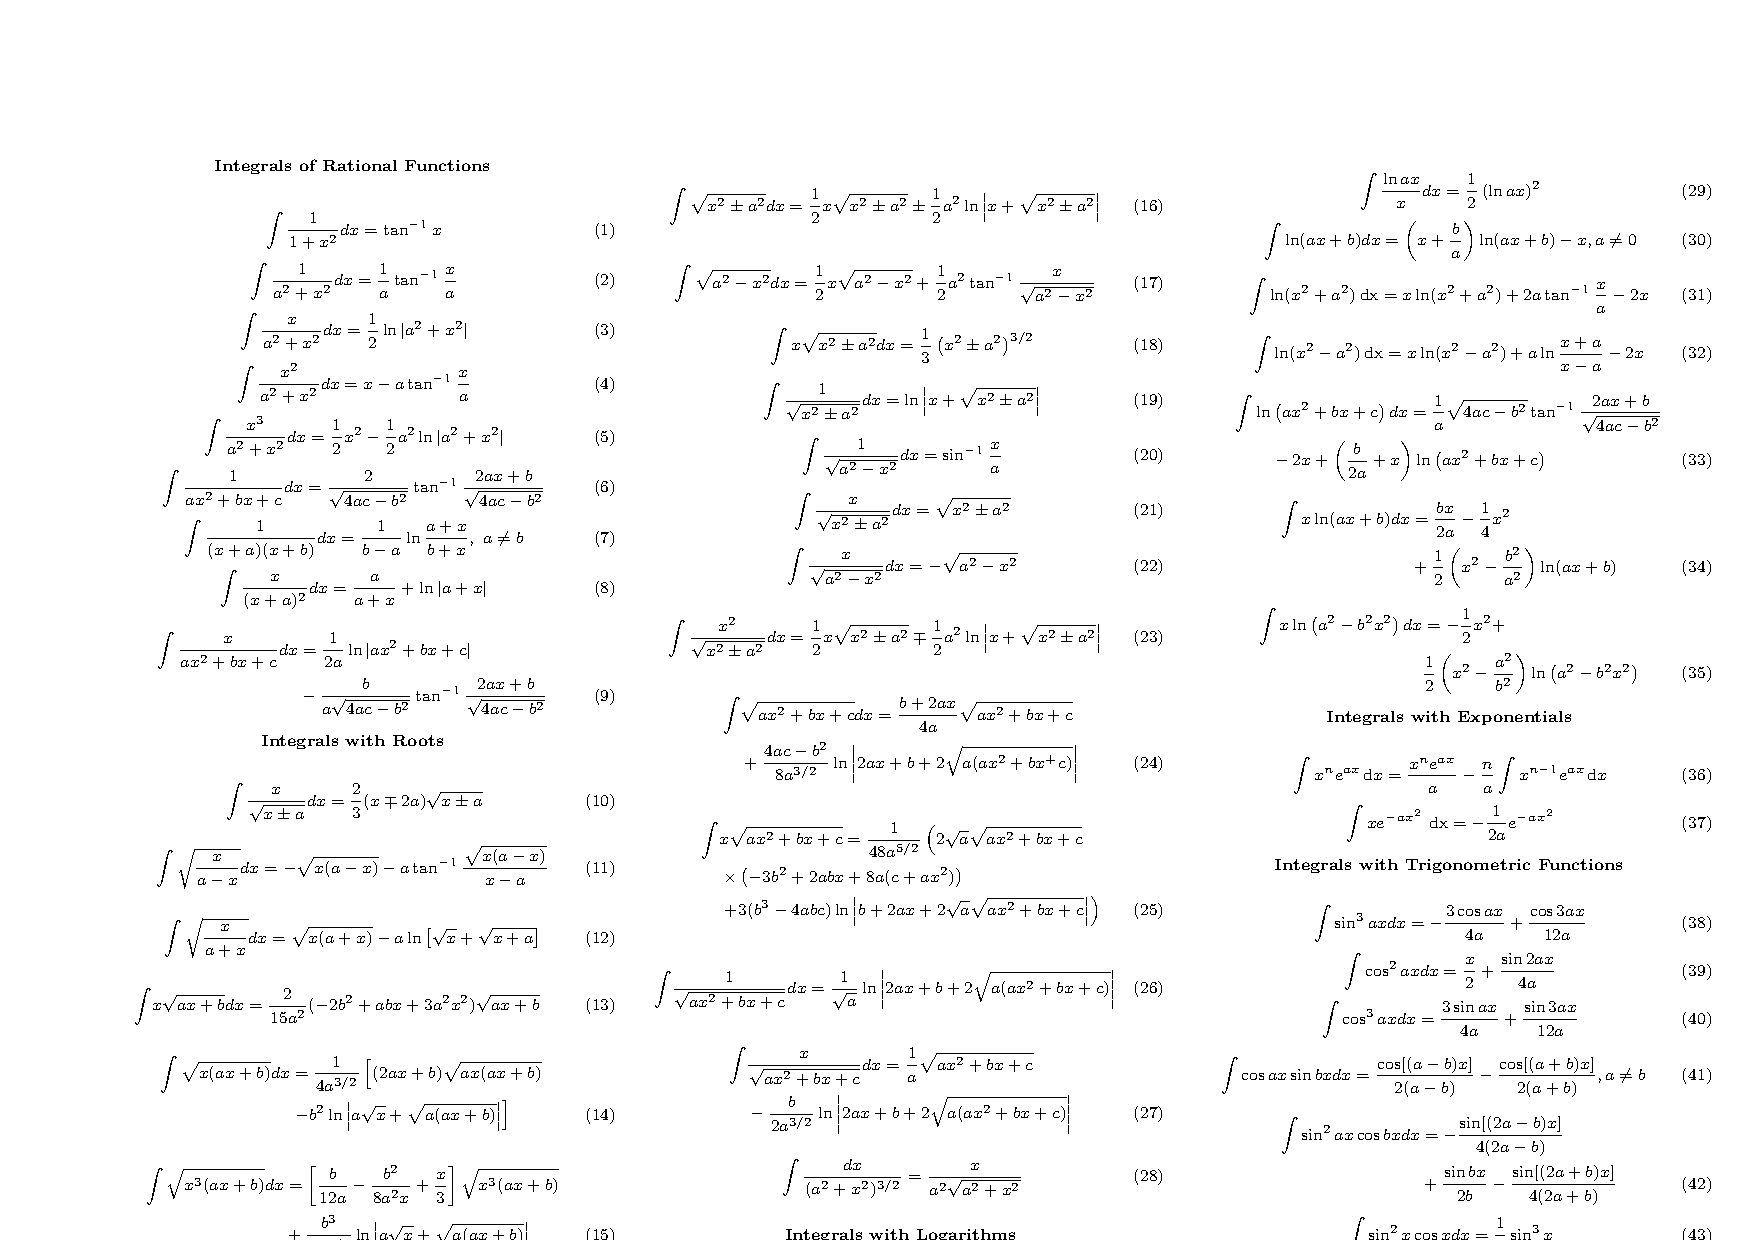
\includepdf[pages={1-2}]{\source/hints/Integral.pdf}

\section{Java}
\inputminted{java}{\source/hints/template.java}
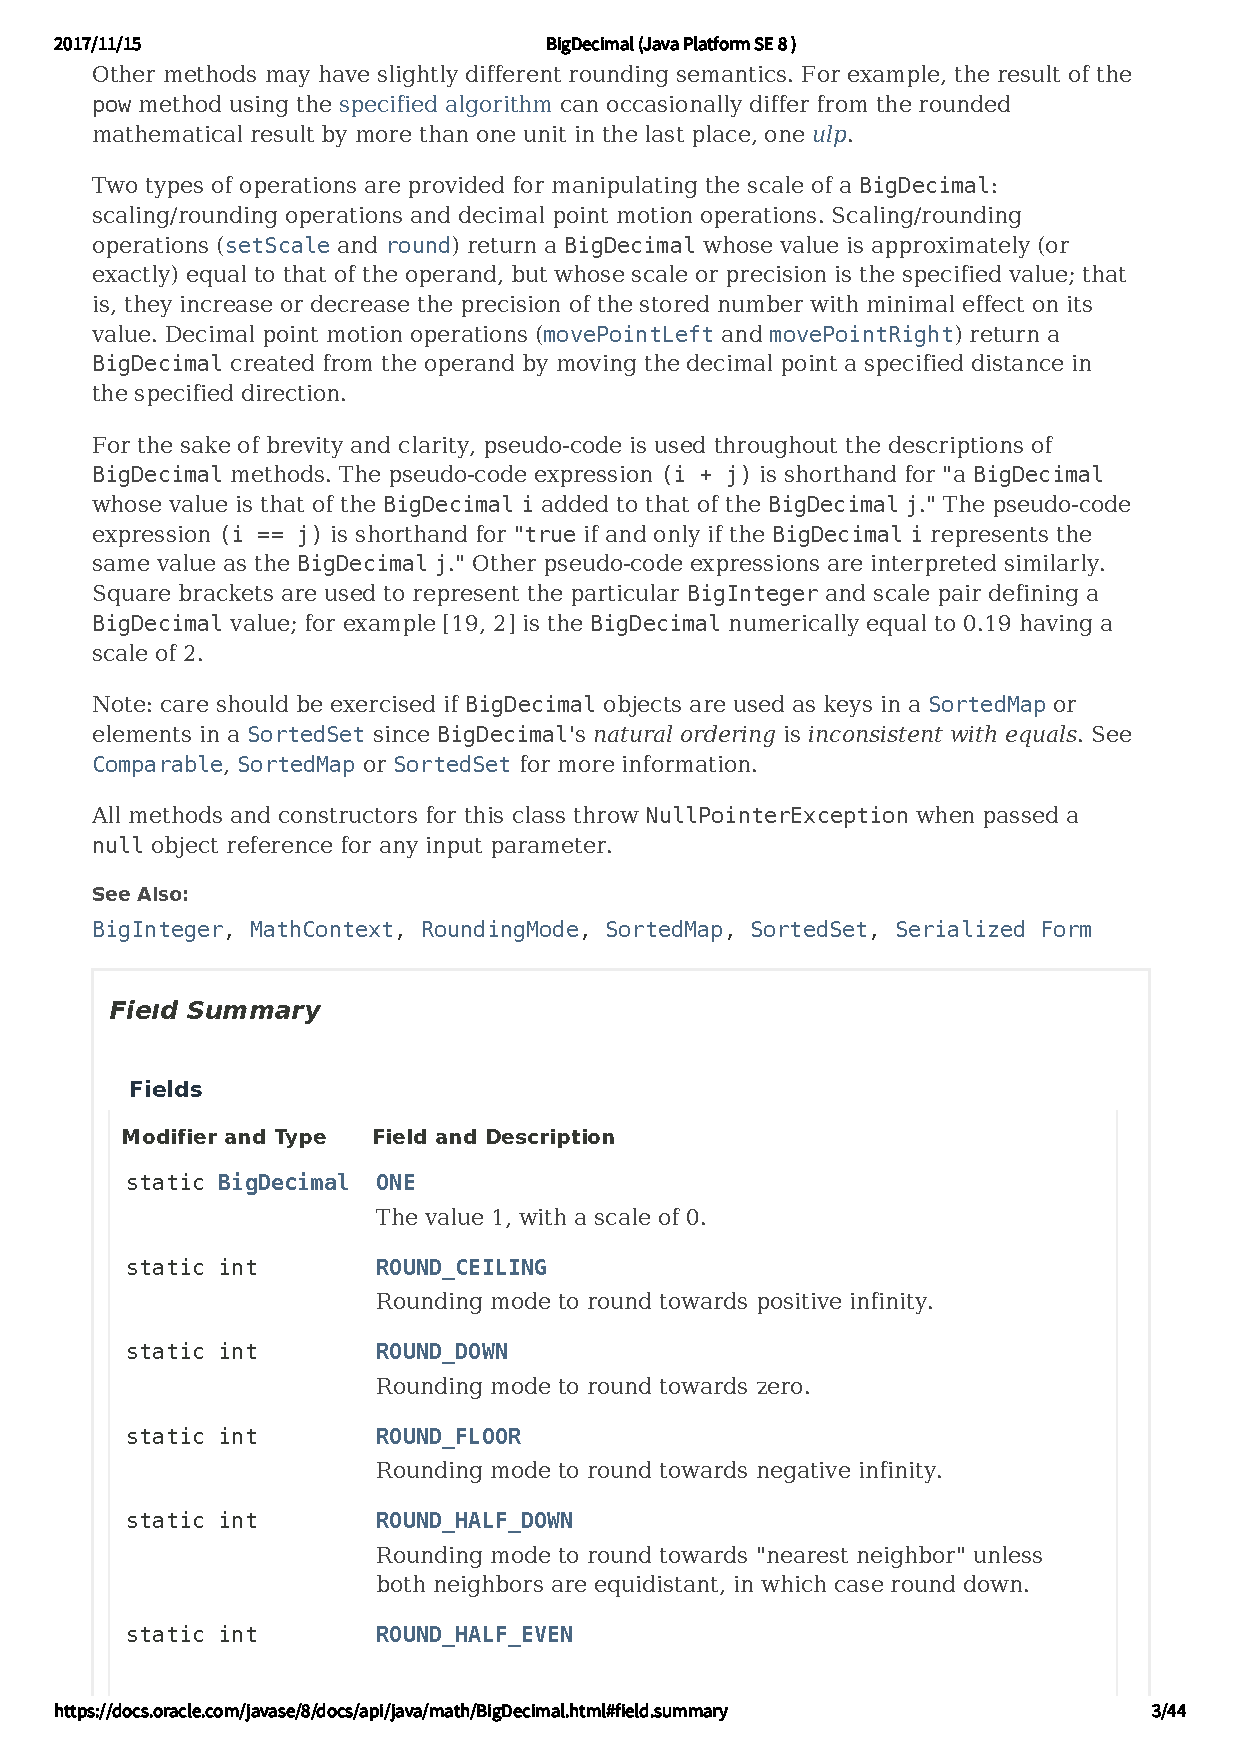
\includepdf[pages={1-6}]{\source/hints/BigDecimal.pdf}
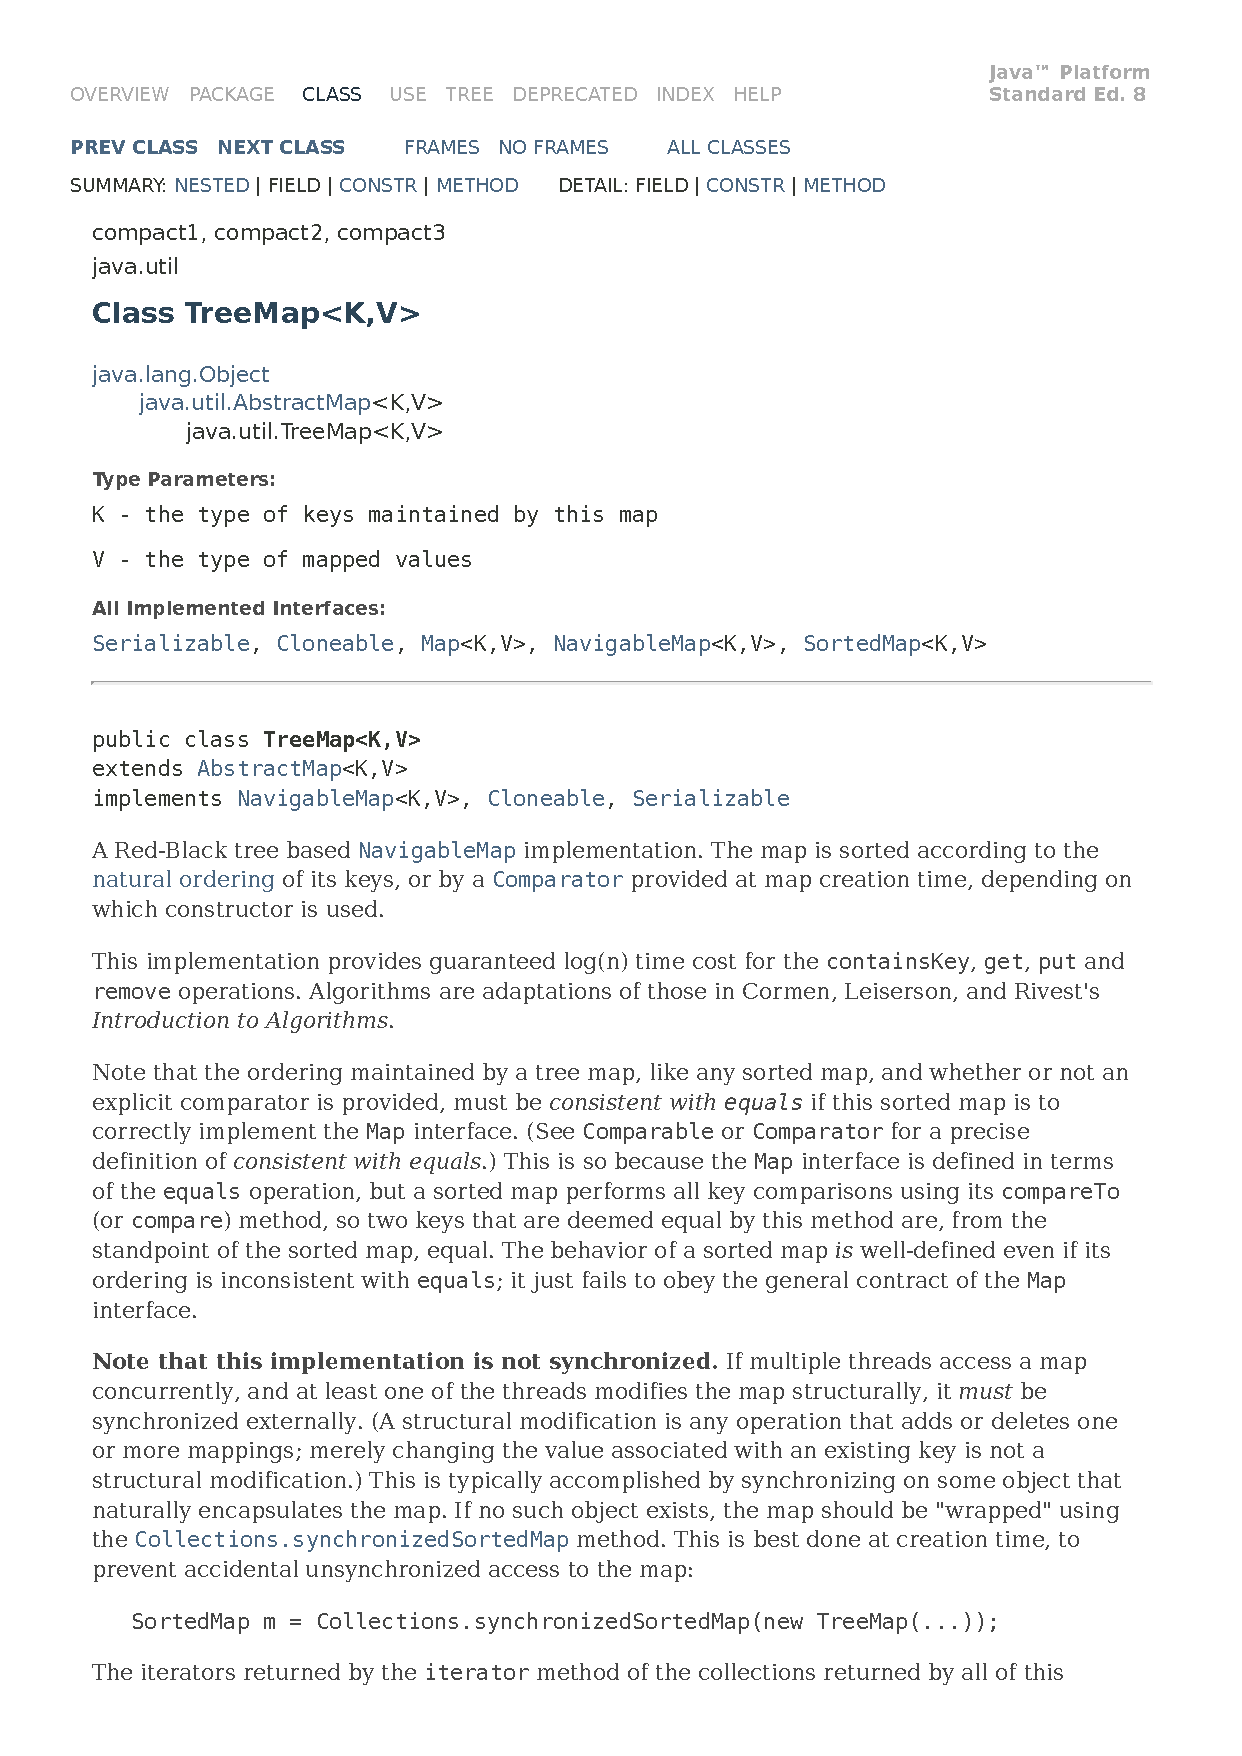
\includepdf[pages={1-5}]{\source/hints/treemap.pdf}
\cleardoublepage
	\end{spacing}
\end{document}
